\documentclass{article}
\usepackage[utf8]{inputenc}

\title{Graph Kernels and Support Vector Machines for Pattern Recognition}
\author{\textbf{Léo Andéol}\thanks{leo.andeol@gmail.com}\\ Master DAC, Sorbonne Université\\ Paris, France\\\\ \footnotesize Supervised by: Prof. Hichem Sahbi}
\date{May 2019}

\usepackage[square,sort,comma,numbers]{natbib}
\usepackage{graphicx}
\usepackage{amsmath,amsthm,amssymb}
\usepackage{mathtools}
\usepackage{multicol}
\usepackage{url}
\usepackage{todonotes}
\usepackage{lipsum}

\DeclarePairedDelimiter{\abs}{\lvert}{\rvert}
\DeclarePairedDelimiter{\norm}{\lVert}{\rVert}

\let\vec\mathbf
\newcommand*{\C}{%
  \mathbb{C}%
}
\newcommand*{\R}{%
  \mathbb{R}%
}
\newcommand*{\Z}{%
  \mathbb{Z}%
}

\newcommand*{\captionsource}[2]{%
	\caption[{#1}]{%
		#1%
		\\\hspace{\linewidth}%
		\textbf{Source:} #2%
	}%
}

\newtheorem{theorem}{Theorem}
\theoremstyle{definition}
\newtheorem{definition}{Definition}

\begin{document}

\maketitle
\begin{abstract}
	The problem of having a framework to classify graphs is becoming increasingly important in the era of data. The issue has been tackled since the beginning of the millennium and there have been significant progress. This report introduces all necessary knowledge to understand the topic and then reviews different graph kernels while focusing on a random walk kernel and its optimization. Some experiments are then conducted to verify the information given by the state of the art, and some attempts are made to accelerate the different methods to compute the kernel.  
\end{abstract}

\newpage

\tableofcontents

\newpage

\section{Introduction}
 \todo{introduction générale plus étendue : 1 et 1/2 page :donner un aperçu/résumé du rapport : un paragraphe par élément - ECRIRE A LA FIN}
 \paragraph{}Nowadays the world is shifting towards a new era where data is the most valuable resource, and researchers are working on algorithms to exploit it the best possible way. Most research is currently focused on the so-called "big data", huge quantities of data which are very sparse and of poor quality. However, there also exist structured databases of good quality, in the form of graphs, this very form being the one studied throughout this project. Graphs can be very useful in various fields, but are partly known for their use in biology, as they can be used to represent proteins or other types of molecules.
 \paragraph{}Classification of such graphs is an important problem of pattern recognition which affects a lot of sectors such as medicine, biology, and more. It was studied since the beginning of the millennium and significant progress has been made : several methods were discovered and gave good results but met a big issue, the complexity of these methods. Indeed, they do not scale well to large graphs as their complexity tends to be several times polynomial. Since then, the main objective of research on this topic has been to either find more computationally efficient algorithms, or to find methods to accelerate the ones already in use.
 \paragraph{}The first part of this report will introduce all the necessary background knowledge which are graphs as already mentioned, but also Support Vector Machines (SVMs) which is a powerful classification algorithm, and kernels which are transformations of data usually used to increase the accuracy of SVMs. However, graphs being non-vector data, kernels have also the purpose of becoming a metric of comparison between two instances of graphs. Thus, the main principles of graph kernels will be introduced as well as their definitions. Afterwards, the different methods used to improve the computation complexity of the kernel will be introduced together with their own complexities, advantages and disadvantages.

\paragraph{}The second part of this report will be focused on the technical side and experiments conducted during the project. A synthetic graph database made of toy data was required to conduct simple and quick experiments. Indeed, it was made in order to verify the claims made in the main publication studied thanks to easy control on matters such as labeled and unlabeled graphs, and variations of the size of either the database or the graphs inside of it. Different challenges and problems met during the implementation will be explained, as well as their solution, if one has been found. Then, the main subject of this part will be discussed : the accuracy and computation time of different methods, estimation of their complexities and different attempts to approximate those methods. Finally, an experiment on a real database of proteins\todo{voir si j'en fait plus} is conducted, and the results analyzed.
 
\section{Methodology}
\subsection{Background}
\subsubsection{Graphs}
\todo{Revoir toutes les refs}
\paragraph{Definition}
A graph\cite{bondy1976graph} is a type of mathematical structure that represents connections between objects. It is more precisely an ordered pair $G=(V,E)$ of two sets: vertices $V$ (or nodes) and edges $E$ that connect two vertices together.
\begin{equation}
	E \subseteq \{(u,v) : (u,v) \in V^2\}
\end{equation}
Vertices represent objects and are usually depicted as circles or spheres whereas edges link pairs or vertices. 
\begin{figure}[!htb]
\begin{multicols}{2}
    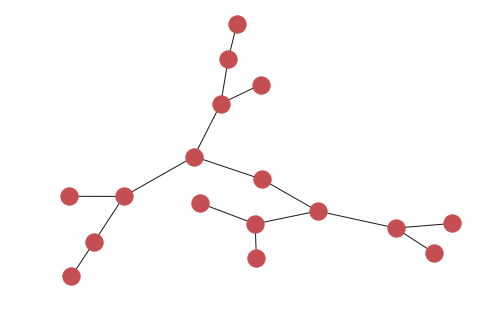
\includegraphics[width=\linewidth]{data/graphs/big_graph_no_label.png}\par
    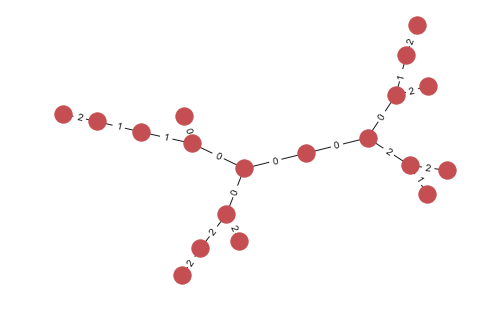
\includegraphics[width=\linewidth]{data/graphs/big_graph_label.png}\par
\end{multicols}
\caption{Two "tree" graphs, resp. unlabeled and labeled}
\end{figure}
\paragraph{Properties} Graphs have a lot of properties that will be used in the rest of this project and will be introduced here
\begin{itemize}
	\item A graph if undirected if and only if : $\forall (u,v) \in E \implies (v,u)\in E$
	\item $\abs{V}$ is the number of vertices and $\abs{E}$ the number of edges
	\item The degree of a vertex $d(v)$ is the number of vertices it is connected to, or the number of distinct edges connected to it.
	\item A path is a sequence of connected edges linking distinct vertices.
	\item A cycle is a path where the first and last vertex is the same.
	\item A graph can have labels (sometimes called colors) either on its vertices or edges (or both). they can take various forms such as being integers, more generally elements of a finite or infinite set and even continuous (such as $\in \R$). 
	\item A graph is said to be connected if all vertices are connected by a path with any other vertex.
	\item A graph is said to be a tree if it is connected and doesn't have any cycle.
	\item A dual graph $G'=(V',E')$ of a graph $G=(V,E)$ is composed of a set of vertices $V'$ of a new vertex for each unique $e\in E$ and a set of edges $E'$ where there is an edge $(u,v)\in V'^2$if and only if there was a vertex connecting the two former edges u and v together.
	\item A subgraph $G'=(V',E')$ of a graph $G=(V,E)$ is that graph restricted to a subset of nodes $V' \in V$ while keeping all the edges with those vertices $E' = \{(u,v) : (u,v) \in E \land (u,v) \in V'^{2}\} \subseteq E$
\end{itemize} Our methods are focused on undirected unlabeled graphs, and undirected graphs labeled by finite sets. Moreover, only edge-labeled graphs will be studied thus if a graph if node-labeled, simply taking its dual graph will do.
\paragraph{Adjacency Matrix} The adjacency matrix of an undirected graph represents the presence or absence of an edge between two specific vertices. It is defined as the matrix $A$ of dimension $\abs{V}\times\abs{V}$ where entries are given by
\begin{equation}
	A_{i,j}=\left\{
	\begin{matrix}
	1 & \mbox{if } i \neq j \mbox{ and } (i,j) \in E \\
	0 & \mbox{otherwise}
	\end{matrix}
	\right.
\end{equation}

\paragraph{History} Graphs were first used in their modern form to represent the problem of Seven Bridges of Königsberg (cite), and have been ever since used to represent maps, and thus path-finding algorithms were developed. They have also been used to represent flow problems, scheduling problems, networking routing and many others(cite). Graphs can also be used, with labels, to represent different types of molecules and interactions between them, or more simply to represent molecules by considering atoms as vertices and bonds as edges.\\
The next part will introduce Support Vector Machines, the algorithm used in this project to classify new unknown graphs into known categories. It has been shown(cite) that it can be used effectively on proteins and enzymes.

\subsubsection{Support Vector Machines}
Support Vector Machines (SVMs)\cite{burges_tutorial_1998} are a type of machine learning algorithms discovered in the early 90s\cite{cortes_support-vector_1995}. It was originally a classification algorithm however it has been expanded since to regression and clustering too. 
\paragraph{Classification}
Classification is one of the two problems of supervised learning that aims to automatically recognize and classify observations $\vec{x}$, such as recognizing handwritten digits. It can be split into two tasks where the first task is to learn from training data how to decide in which class (or group) to classify an example from its attributes and the second is to predict the class of new examples. All of that, while minimizing errors. This problem can be formalized as\todo{Parler de la theorie de l'apprentissage ? risque structurel etc ? et dire quelle loss on utilise ou pas ?}
\begin{definition}
	Classification is the problem of finding the best function $f :  \R^d \longrightarrow \{0..k\}$ among a set of functions $F$ while minimizing a risk function $R$
	\begin{equation}
		f\star = \mbox{argmin}_f R(f)
	\end{equation}
	 where $k$ is the number of classes of the problem and $d$ the number of features of data 
\end{definition}
SVMs are especially powerful at this task and widely used for the two following reasons.
\paragraph{Margin and support vectors}
The Support Vector Machines are based on the model of the Perceptron\cite{freund1999large}, another classification algorithm that tried to find an hyperplane that discriminates the two sets.The main issue with the Perceptron is that it had no formal guarantee to find an optimal hyperplane, and more often than not would not find it. Moreover, if the data weren't linearly separable, the algorithm would not converge.\\
In order to tackle theses issues, the SVM offered three fixes. First, a margin was added in the loss $L$ function in order to not only classify well the data samples, but also with the maximum certainty, i.e. as far from the decision boundary as possible.
\begin{equation}
    L(y_i ,\vec{x}_i,w) = \max(0,-y_i \vec{x}_i \cdot w + w_{0}) \implies L(y_i ,\vec{x}_i,w) = \max(0,1-y_i \vec{x}_i\cdot \vec{w} + w_{0})
\end{equation}
Where $x$ is the features vector of an instance, $y$ its class and $\vec{w}$ and $w_{0}$ respectively the weight vector and bias calculated by the algorithm.
Then, seeing this solution wasn't enough, as there was still an infinity of possible solutions, it was proven that the margin $\gamma$ between points and the decision boundary was inversely proportional to the norm of the weights.\\
\begin{equation}
\gamma_i = \frac{y_{i}(\vec{x}_{i} \cdot \vec{w} + w_{0})}{\norm{\vec{w}}}
\end{equation}
These two fixes gave us the first version the SVM, the hard-margin SVM\\ 
\begin{equation}
    \min \frac{1}{2}\norm{\vec{w}}^{2} \quad
\textup{s.t.}\quad y_{i}(\vec{x}_{i} \cdot \vec{w} + w_{0}) \geq 1 \quad \forall i \in \{1..n\}
\end{equation}
However, if the data weren't linearly separable the algorithm wouldn't be optimizable since the quadratic programming problem requires all points to be correctly classified. Then, a new term $\xi$ was introduced as an error tolerance, as well as a factor $C$ that would determine the balance between error tolerance and weights minimization.\\
\begin{equation}
\begin{array}{ll@{}ll}
\text{min}  & \frac{1}{2}\norm{\vec{w}}^{2}+C\sum\limits_{i=1}^{n}\xi_{i} &\\
\text{s.t.}& \forall i \in \{1..n\} & y_{i}(\vec{x}_{i} \cdot \vec{w} + w_{0}) \geq 1-\xi_{i}
\end{array}
\end{equation}
Then, the next section will introduce the second advantage of SVMs.
\subsubsection{Kernels}
In its dual form, the SVM problem only requires a dot product between the sample vectors. 
\begin{equation}
	\begin{array}{ll@{}ll}
	\text{max} & \sum\limits_{i=1}^{n} \alpha_i - \frac{1}{2} \sum\limits_{j=1}^{n}\sum\limits_{i=1}^{n}\alpha_{i}\alpha_{j}y_{i}y_{j}\vec{x_{i}}^{\top}\vec{x_{j}}\\
	\text{s.t.} & \forall i\qquad 0 \leq \alpha_{i} \leq C\\
	& \qquad \;\; \sum\limits_{i=1}^{n} \alpha_{i}y_{i}=0
	\end{array}
\end{equation}
Where $n$ is the number of instances.
Then, a nonlinear transformation $\phi(x)$ can be used to replace the dot-product $\vec{x}_i \cdot \vec{x}_j$ by $\phi(\vec{x_{i}})\cdot\phi(\vec{x}_{j})$ , effectively augmenting the size of our vectors and thus the expressiveness of our model by enhancing the separability of the data. However, for complex transformations, such as in infinite dimensions, the function $\phi$ isn't defined. But it was found that the standard dot product can be replaced by another function as long as it is a bilinear positive semi definite form. 
\begin{definition}
	A kernel $K$ is positive semi definite if and only if\\
    \begin{equation}
    	\sum\limits_{i=1}^{n}\sum\limits_{i=1}^{n}\kappa(\vec{x_{i}},\vec{x_{j}})c_{i}c_{j} \geq 0 \qquad \forall i \in \{1..n\} \quad c_i \in \R
    \end{equation}
\end{definition}
Thus, the dot product can be replaced by a function $K(x_1,x_2)$ which will indirectly map the data to higher dimensions, even infinite with the RBF kernel and return the dot product of those transformations, while remaining computable in all cases. This replacement is usually called the Kernel Trick.
Ever since the foundation of SVMs, the kernel trick became a big focus of the machine learning community as it naturally fits in the algorithm and allows supervised learning on very complex data, and enjoying greater accuracy than most algorithms.\todo{Est-ce qu'il faut rentrer dans le détail ? rajouter quoi?}\\
The fact that the dot product can be replaced by a function without specifying the map $\phi$ is the reason why the Kernel Trick became a big focus of research. In particular, it will be possible to make a kernel for non vector data such as graphs, as shown in the next section. 
\subsection{State of the Art}
This section will review the state of the art kernels for graphs. Particular attention will be given to the random walk kernel.
\subsubsection{Graph Kernels}
Graph Kernels are a type of R-convolution kernels\cite{haussler99convolution} applied to graphs, which are kernels that are based on decompositions of complex objects and comparisons of those decompositions.\\
Graph Kernels have been studied since Support Vector Machines started getting popular\cite{kashima_graphkers_2003}. Since then, a lot of progress has been made, and several types of kernels have been discovered, such as random walk and graphlet\cite{shervashidze_efficient_2009} kernels, the two main families of kernels (and the ones studied in this section), but not the only ones.
There are also graph kernels that use subtrees\cite{ramon2003expressivity}, shortest paths\cite{borgwardt2005shortest} and several others that are unfortunately usually  either too complex to compute or not positive semi-definite\cite{shervashidze2012scalable}. However it has been shown\cite{schlkopf_learning_2001} that in some cases non positive semi definite kernels can still be used efficiently either by using them as a dissimilarity measure. They can also be artificially made positive semi definite.\todo{developper plus les autres graphes?}
\subsubsection{Graphlets}
A graphlet is a non-empty graph of $k=3$, $4$ or $5$ nodes. The idea of the graphlet kernel $\kappa$ is to generate a set $S$ all possibles graphlets of a certain size $k$ and calculate for each of them the frequency of occurrence in a certain graph $G=(V,E)$ to build a vector $\vec{f}_G$ of size $\abs{S}$. The kernel is then defined as follows
\begin{definition}
	Let $G$ and $G_2$ be two graphs, $\vec{f}_G$ and $\vec{f}_{G_2}$ the frequency vectors of respectively $G$ and $G_2$, then the kernel $\kappa$ is defined as
	\begin{equation}
		\kappa(G,G_{2})=\vec{f}_{G}^{\top}\vec{f}_{G_2}
	\end{equation}
\end{definition}
However the complexity of this calculating a vector $\vec{f}_G$ is $O(n^k)$ where $n=\abs{V}$ and is thus computationally extremely expensive. In order to address this issue, a sampling method was introduced. Indeed, if enough samples are drawn, the Law of Large numbers indicates that the sampled distribution will converge to the actual (theoretical) distribution. However a bound has been found on the complexity of such sampling\cite{weissman2003inequalities} allowing better precision.
\subsubsection{Random walks}
Graph kernels based on Random Walks have been studied since very early\cite{kashima_graphkers_2003}, several of them were created and were then united\cite{vishwanathan_graph_2010}. Random walks are a type of rather intuitive algorithms : the idea is to randomly walk through a graph and then compare it to random walks in another graph. Actually, all the random walks are computed at the same time by making the adjacency matrix stochastic by dividing each column of the matrix by its sum (normalizing it) and using it as a Markov chain.\\
Moreover, it has also been shown\cite{imrich2000product} that performing a walk on two separate graphs at the same time is the same as performing a walk on the product graph. The product graph is in simpler terms the Cartesian product of the two graphs, taking all possible combinations of nodes and linking those nodes when there is an edge between two specific nodes in both the original graphs. \\
\begin{definition}
	Let $G_1=(V_{1},E_{1})$ and $G_2=(V_{2},E_{2})$ be two graphs,\\the product graph
	$G_\times = (V_{\times},E_{\times})$ is then defined as
	\begin{itemize}
		\item $V_{\times} = \{(v,w) : v \in V_{1}, w \in V_{2} \}$
		\item $E_{\times} = \{((v_1,w_1),(v_2,w_2)) : v_1,v_2 \in V_{1}^2, w_1,w_2 \in V_{2}^2 \}$
	\end{itemize}
\end{definition}

However, technically, the adjacency matrix $W_{\times}$ of a such graph is the result of the Kronecker (tensor) product of the two adjacency matrices $A$ and $A_2$ of the two graphs \cite{weichsel1962kronecker}
\begin{equation}
    W_{\times}=A \otimes A_{2}
\end{equation}
In case the graphs are labeled, then the adjacency matrix $W_{\times}$ is the sum of the Kronecker products of adjacency matrices restricted to each label $l$ 
\begin{equation}
	W_{\times}=\sum\limits_{l=1}^{d} A_1^{(l)} \otimes A_2^{(l)}
\end{equation}
Where $d$ is the size of the label set and $A_x^{(l)}$ the adjacency matrix of $G_x$ restricted to the label $li$ which is defined as follows
\begin{equation}
	A^{(l)}=\left\{
		\begin{matrix}
		1 & \mbox{if } i \neq j \mbox{ and } (i,j) \in E \mbox{ and } (i,j) \mbox{ is labeled } l\\
		0 & \mbox{otherwise}
		\end{matrix}
		\right.
\end{equation}
The $vec$ operator will also be used as it is very linked to the tensor product. It is the vector obtained by stacking all columns of $A$.

\paragraph{Kernel definition}
The idea of the kernel is to perform random walks simultaneously on two graphs in order to compare the walks they have in common. As shown above, that can be achieve by simply performing a random walk on the product graph. 
By making the adjacency matrix stochastic, and computing the $k$-th power of the matrix $W_\times$, the probabilities obtained are the ones of walks in common (starting and ending at the two same nodes) between the two graphs of length $k$.
By taking into account the start $p_\times$ and end $q_\times$ probabilities, the sum of paths of all possible length can be calculated. Moreover using a power series $\mu(k)$ helps de-emphasizing longer walks and makes the sum converge. 
\begin{definition}Let $p_{\times}$ and $q_{\times}$ be respectively the start and end probability of each node, and let $W_{\times}$ be the adjacency matrix of the product graph of $G$ and $G'$, and finally $\mu(k)$ be a convergent function of $k$.
	\begin{equation}
		\kappa(G,G') = \sum\limits_{k=0}^{\infty}\mu(k)q_{\times}^{\top}W_{\times}^{k}p_{\times}
	\end{equation}
\end{definition}
This kernel can be computed in $O(kn^6)$ where $k$ is the number of iterations 
\paragraph{Inverse Kernel}
There is a specific case of the kernel following provided a power series is used. Indeed, by replacing the power series as follows $\mu(k)=\lambda^k$ the following kernel is obtained 
\begin{equation}
	\kappa(G_1,G_2)=q_{\times}^{\top}(I-\lambda W_\times)^{-1}p_{\times}
\end{equation}
It can also be computed in $O(n^6)$ however in practice the hidden factor is much lower which makes it a better option for very small graphs and databases and the accuracy much better since there isn't any tradeoff on the number of iterations. Moreover, it will inspire some of the following methods.
\paragraph{Sylvester Equation}
A Sylvester equation, also sometimes called Lyapunov equation is a matrix equation of the following shape 
\begin{definition}
	Let $A$, $B$, and $C$ be matrices of compatible shapes, then the Sylvester equation is
	\begin{equation}
	AX+XB=C
	\end{equation}
	And the discrete-time Sylvester Equation is 
	\begin{equation}
	AXB+C=X
	\end{equation}
	Which can be generalized as
	\begin{equation}
		\sum_{i=0}^{d}A_{i}XB_{i}=X
	\end{equation}
\end{definition}
We will be exclusively using the discrete-time Sylvester Equation and its generalization and will be referring to it as Sylvester equation. These equations are solved usually using Schur decompositions in $O(n^3)$ for the basic Sylvester equation and in unknown time for the generalized version\cite{vishwanathan_graph_2010}.\\
We can use this equation to solve our kernel faster if we assume a geometric function $\mu(k)=\lambda^k$ with $\lambda$ an hyperparameter. It can be achieved by replacing the $A$ and $B$ matrices by our adjacency matrices $A_1$ and $A_2$, adding $\lambda$, and $C$ by our start probabilities $p_\times$ while vectorizing the whole equation thus obtaining
\begin{equation}
	vec(M) = vec(\lambda A_{1}MA_{2}) + p_{\times}
\end{equation}
From which we can obtain (where I is the identity matrix)
\begin{equation}
	q_{\times}^{\top}vec(M)=q_{\times}^{\top}(I-\lambda W_{\times})^{-1}p_{\times}
\end{equation}
Thus, having calculated the inverse kernel by an alternative method. The advantage of this method is that it is very fast, but unfortunately limited to unlabeled graphs, unless there is an implementation for the generalized Sylvester equation. Moreover, compared to the others, this option is very simple and does not require specific parameters, but like many others, suffers when it encounters singular matrices. 
\paragraph{Conjugate Gradient Method}
The Conjugate Gradient Method\cite{nesterov_lectures_2018} is an optimization algorithm used to find approximate solutions of linear systems that have a positive semi definite matrix. As its name suggests, it is a gradient based iterative algorithm. The Main idea is that normal gradient descent only takes into account the gradient at the current step of the algorithm, and depending on the step size may cancel progress made in the previous step.
\begin{figure}[!htb]
	\centering
	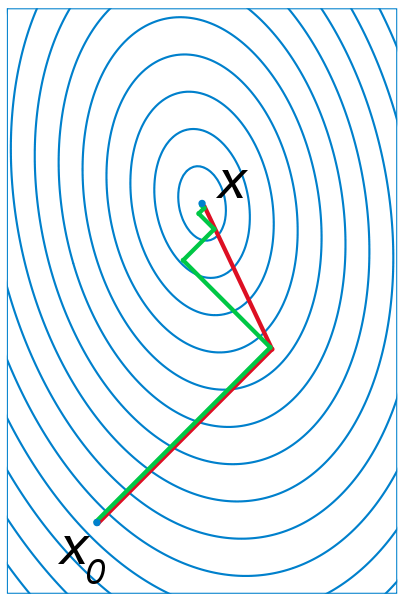
\includegraphics[height=0.3\textheight]{data/sota/conj_grad.png}
	\caption{Conjugate gradient (red) compared to Gradient Descent (green)}
	\label{fig:conj_grad}
\end{figure} 
The Conjugate Gradient method was introduced as a fix for that issue. The idea of the algorithm is to keep the former gradients in order improve the convergence speed by making the new gradient orthogonal to all the former one through the Gram-Schmidt process, at each step. Thus, unless there are approximation errors, the algorithm guarantees converge in $n$ steps, being the number of dimensions of the problem, here the size of our graph.\\
However, this algorithm has limitations, it can only be used to solve linear systems of equations as $Ax=b$ under the constraint that $A$ is symmetric positive definite.
In our case, this algorithm can be used to solve the following problem 
\begin{equation}
	(I-\lambda W_{\times}x=p_{\times}
\end{equation}
And the kernel value can be obtained by computing $q_{\times}^{\top}x$. The complexity of that method is $O(rn^3)$ for unlabeled graphs and $O(rdn^3)$ for labeled graphs where $r$ is the effective rank of the matrix $W_{\times}$. It is important to note that this kernel also assumes a geometric $\mu(k)$ function. \\
This method is thus more slow than the Sylvester Equation, however it is easily applied to labeled graphs, which is its main advantage.
\paragraph{Fixed Point Iterations}
A fixed point is a value for which a function, returns that same value 
\begin{definition}
	Let $S$ a set and $f$ a map $f : S \implies S$,\\
	$x \in S$ is a fixed point of $f$ if and only if $x=f(x)$ 
\end{definition}
Fixed point iterations is a method of computing a fixed point of a function by applying repeatedly the following equation until $\norm{x_{n+1}-x_{n}}<\epsilon$ where $\epsilon$ is the acceptable level of error.
\begin{equation}
	x_{n+1} = f(x_n)
\end{equation}
There is also a guarantee of convergence 
\begin{theorem}
	In order for the fixed-point iterations to converge, it is necessary that $\lambda<|\xi|^{-1}$ where $\xi$ is the largest eigenvalue of $W_\times$
\end{theorem}
\todo{le mettre en appendix?}
\begin{proof}
  Let $x_0=p_\times$ and $t>>0$
  \begin{align*}
      x_{t+1}-x_t &= p_\times+\lambda W_{\times} x_t - x_t &\\
      &= p_{\times}+(\lambda W_{\times} - 1)(p_{\times}+\lambda W_{\times} x_{t-1})\\
      &= p_{\times} - p_{\times} + \lambda W_{\times}p_{\times} + (\lambda W_{\times})^2 x_{t-1} - \lambda W_{\times} x_{t-1}\\
      &= \lambda W_{\times}(p_{\times}-x_{t-1}+\lambda W_{\times} x_{t-1}) \\
      &= \lambda W_{\times}(p_{\times}-\lambda W_{\times} x_{t-2} - p_{\times} + \lambda W_{\times}(\lambda W_{\times} x_{t-2} +p_{\times}) \\
      &= \lambda W_{\times} ( \lambda W_{\times} (\lambda W_{\times} x_{t-2}+p_{\times}-x_{t-2})) \\
      &= (\lambda W_{\times})^2(\lambda W_{\times} x_{t-2}+p_{\times} - x_{t-2}) & \\
      \text{We find a pattern}\\
      \implies x_{t+1}-x_t &= (\lambda W_{\times})^t (\lambda W_{\times} x_0 + p_{\times} - x_0) & \\
      \text{And because } x_0 = p_{\times}\\
      &= (\lambda W_{\times})^{t+1} p_{\times}\\
      \text{Which decreases only when}\\
      \xi_1 < 1\\
      \text{The largest magnitude eigenvalue of} \lambda W_{\times}\\
      \implies \lambda < |\xi_1|^{-1}
      && \qedhere
  \end{align*}
\end{proof}
Since this method requires the computation of $W_\times$, the kernel value can be computed for any type of labeling. For unlabeled graphs, the complexity is $O(kn^3)$ and $O(kdn^3)$ for labeled graphs, where $d$ is the number of labels and $k$ the number of iterations which can be estimated by
\begin{equation}
	k=O\left(\frac{\ln \epsilon}{\ln \lambda + \ln \abs{\xi}}\right)
\end{equation}
Finally, the fixed point iterations is more demanding than the others since it has a condition on the value of $\lambda$ and thus assumes as geometric $\mu(k)$ function, and the number of iterations can easily vary a lot. The only advantage of this method is that it is very simple while still being better than the raw kernel.
\paragraph{Spectral Decomposition}
The Spectral Decomposition, usually called the eigendecomposition of a matrix $M$ is a factorization in the form $VDV^{-1}$ where $D$ is the diagonal matrix of eigenvalues and V the matrix of eigenvectors. This decomposition can reduce the computation time of the kernel by making most of the matrix operations trivial
\begin{equation}
	\kappa(G,G_2)=\sum\limits_{k=0}^{\infty}\mu(k)q_{\times}^{\top}(V_{\times}D_{\times}V_{\times}^{-1})^{k}p_{\times} = q_{\times}^{\top}V_{\times}\left(\sum\limits_{k=0}^{\infty}\mu(k)D_{\times}^{k}\right)V_{\times}^{-1}p_{\times}
\end{equation}
Indeed, the power now only applies to a diagonal matrix which can be computed much faster. Moreover, this method unlike the others preserves the prior $\mu(k)$ without any conditions. If $\mu(k)=\lambda^k$ is chosen then the kernel becomes
\begin{equation}
	\kappa(G,G_2)=q_{\times}^{\top}V_{\times}(I-\lambda D_{\times})^{-1}V_{\times}^{-1}p_{\times}
\end{equation}
That kernel is even more trivial to compute as the inverse of a diagonal matrix is simply the inverse of each of its entries and is thus computed in linear time. Finally, by using $\mu(k)=\frac{\lambda^k}{k!}$  as prior, the following new kernel is obtained
\begin{equation}
	\kappa(G,G_2)=q_{\times}^{\top}V_{\times}{e^{\lambda D_{\times}}}V_{\times}^{-1}p_{\times}
\end{equation}
However, the complexity of the computation of the eigendecomposition is as large as the raw kernel $O(n^6)$, but, for unlabeled graphs, a big improvement is possible by simply calculating the eigendecompositions of the original adjacency matrices $A_1$ and $A_2$ thus cutting the time to $O(n^3)$, thanks to a property of the Kronecker product
\begin{equation}
	A_1 \otimes A_2=(V_{1}D_{1}V_{1}^{-1})\otimes(V_{2}D_{2}V_{2}^{-1})=(V_1\otimes V_2)(D_1 \otimes D_2)(V_1 \otimes V_2)^{-1}
\end{equation}
By rewriting the spectral decomposition kernel taking advantage of this property, the following new kernel is obtained
\begin{equation}
	\kappa(G_1,G_2)=(q_{1}^{\top}V_{1}\otimes q_{2}^{\top}V_{2})(\sum\limits_{k=0}^{\infty}\mu(k)(D_{1}\otimes D_{2})^k)(V_{1}^{-1}p_{1}^{\top}\otimes V_{2}^{-1}p_{2}^{\top})
\end{equation}
Which can also be altered by choosing specific $\mu(k)$ as described above. This method ends up being the most efficient of all for unlabeled graphs as it is computed in $O(pn^3)$ where $p$ is the computation time of the power series $\mu$. Moreover this complexity can further improve the computation time of the gram matrix because the eigendecomposition of an adjacency matrix only needs to be computed once. However, this method cannot be expanded to labeled graphs as it encounters difficulties applying the property mentioned above.
\paragraph{Nearest Kronecker Product Approximation}
This method is more particular as it is not a new way to compute the kernel, but rather a way to generalize all the other methods. Indeed the Nearest Kronecker Product Approximation\cite{van1993approximation} is used to approximate two matrices $A$ and $B$ as if their Kronecker product was equal to the Kronecker product of two labeled graphs' adjacency matrices $W_{\times} \approx A \otimes B$. This methods allows using any of the methods mentioned above since it returns only two matrices and thus brings back the problem to unlabeled graphs. This method tries to minimize the Frobenius norm of the difference between the two $\norm{W_\times - A\otimes B}_F$. It can be computed in $O(dn^2)$ since $W_\times$ is a sum of Kronecker products.\\
However this method also brings its own set of drawbacks. Since it required the Kronecker product of each couple of adjacency matrices to be computed, the previous advantage of the Spectral Decomposition (only computing once the eigendecomposition for each adjacency matrix) is lost as the obtained matrices are unique for each $W_\times$.

\subsubsection{Digest}
\todo{remplir}




\section{Experiments}
\todo{experiences : détailler db, tests, méthodes, les parametres, construction label, donner tableaux, resultats, teps de calculs, précision, discuter tout cela}
A big part of this project consisted in implementing the different algorithms from the main paper that I had studied \cite{vishwanathan_graph_2010}, verifying the results obtained in that article, and making new attempts to accelerate those algorithms while keeping the best accuracy possible.
\subsection{Implementation}
Implementing code from the main paper was a challenge in itself. Several problems aren't really documented and finding functions to solve them, or even explanations on how to solve them is sometimes difficult.
\subsubsection{Graphs}
The first thing that had to be done was to create a graph database generator, of very simple and standard graphs that had expectable behaviors and could thus be used for tests. Those graphs would also be altered using simple transformations, in order to create different graphs belonging to the same class.\\
\begin{figure}[!htb]
	\begin{multicols}{4}
		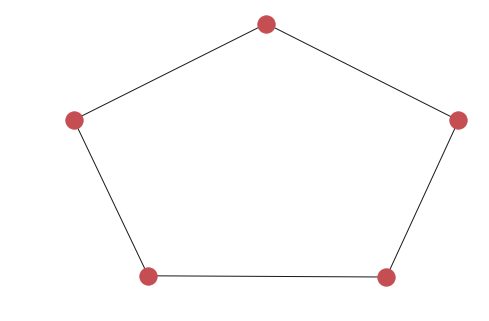
\includegraphics[width=\linewidth]{data/generated-graphs/ring_base.png}\par
		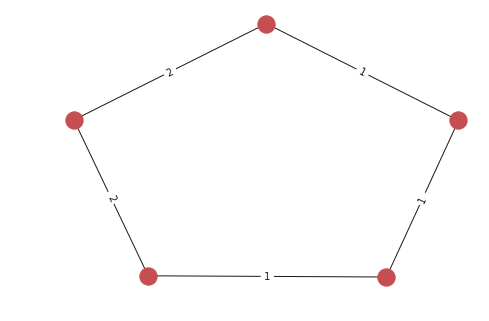
\includegraphics[width=\linewidth]{data/generated-graphs/ring_labels.png}\par
		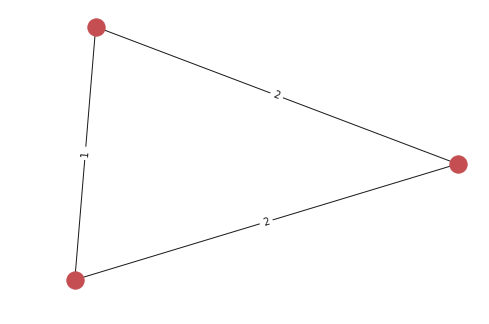
\includegraphics[width=\linewidth]{data/generated-graphs/ring_altered_struct.png}\par
		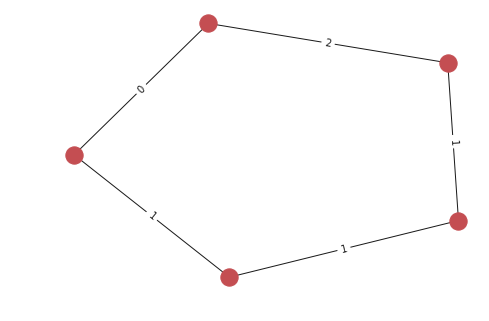
\includegraphics[width=\linewidth]{data/generated-graphs/ring_altered_labels.png}\par
	\end{multicols}
	\caption{Ring graphs, resp. unlabelled, labelled, altered structured, altered labels}
\end{figure}
For simplicity, it was decided to only use 3 classes to stay as simple as possible. We studied 3 standard types of graphs : the ring, the star and the tree. A ring graph is a connected graph where each vertex is connected to exactly two vertices, it thus forms one big cycle. A star graph is composed of a central node, and of several other nodes that are all and only connected to the central node, it should look like a star, or perhaps a flower.\todo{Est-ce que je devrais dire ça ?}. Finally, a tree is a famous type of graph : it is a connected graph without any cycles, but here we will be studying a special type of tree, since each vertex is at most of degree 3.\\
\begin{figure}[!htb]
	\begin{multicols}{4}
		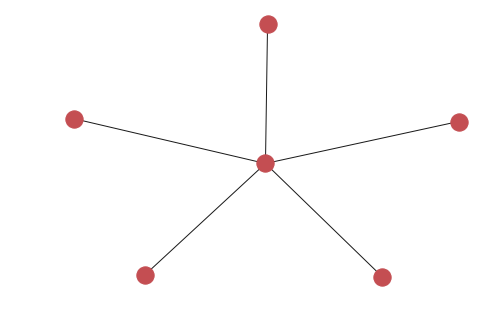
\includegraphics[width=\linewidth]{data/generated-graphs/star_base.png}\par
		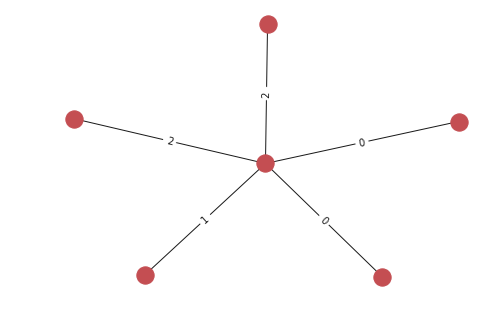
\includegraphics[width=\linewidth]{data/generated-graphs/star_labels.png}\par
		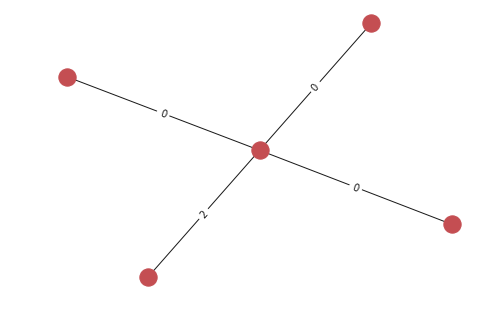
\includegraphics[width=\linewidth]{data/generated-graphs/star_altered_struct.png}\par
		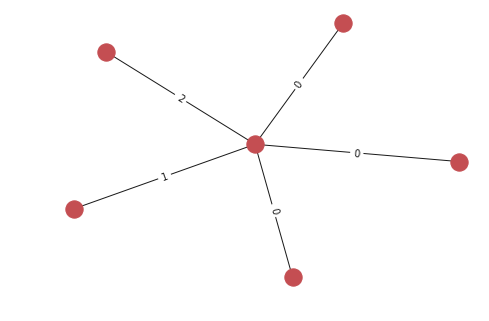
\includegraphics[width=\linewidth]{data/generated-graphs/star_altered_labels.png}\par
	\end{multicols}
	\caption{Star graphs, resp. unlabelled, labelled, altered structured, altered labels}
\end{figure}
The database generator works as follows:\todo{verifier si anglais, et c'est ok mettre deux points ?} for each type of graph, it will create a graph of predetermined size with randomly generated edge labels in a certain given interval. Then, for each graph, it will alter it a predefined number of times, and each time will create a new graph that has been both altered on structure and on labels. Alteration on structure involves removing or adding a predefined number of nodes in respect of the type of the graph thus staying in the same class as the source. 
\begin{enumerate}
	\item Ring graphs are simply regenerated slightly longer or shorter randomly.
	\item Star graphs are also regenerated either with more or less nodes, randomly.
	\item Tree graphs are either expanded by adding randomly leaves anywhere in the graph, or reduced by randomly removing leaves.
\end{enumerate}
Alteration on labels will randomly switch a predefined\todo{predefined beaucoup répété, c'est un probleme ?} number of edge labels. Once this is done, the generator will create two databases out of the set of previously generated graphs, one will be made of the adjacency matrix of each graph without looking at labels, and the second one will be an array of adjacency matrices taken from graphs induced by selecting only edges with a specific label, and that for all labels in the label set.
\begin{figure}[!htb]
	\begin{multicols}{4}
		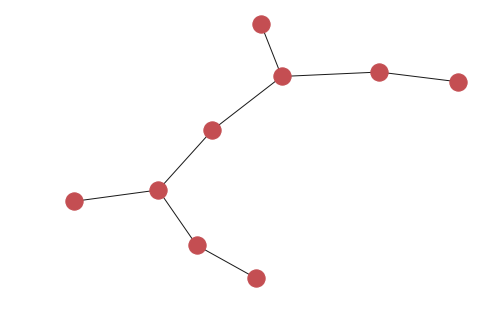
\includegraphics[width=\linewidth]{data/generated-graphs/tree_base.png}\par
		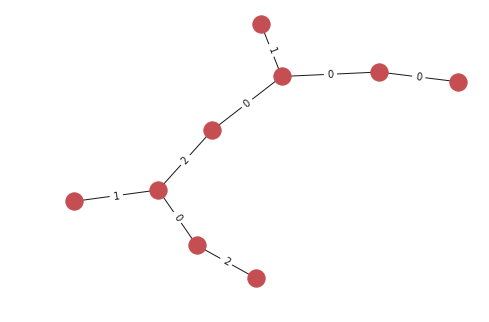
\includegraphics[width=\linewidth]{data/generated-graphs/tree_labels.png}\par
		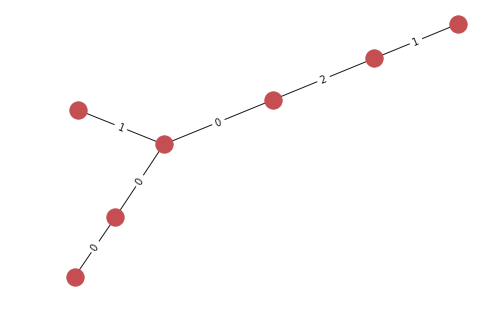
\includegraphics[width=\linewidth]{data/generated-graphs/tree_altered_struct.png}\par
		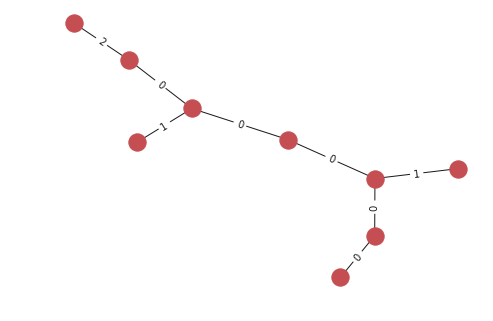
\includegraphics[width=\linewidth]{data/generated-graphs/tree_altered_labels.png}\par
	\end{multicols}
	\caption{Tree graphs, resp. unlabelled, labelled, altered structured, altered labels}
\end{figure}
\subsubsection{Raw Kernel}
\subsubsection{Inverse Kernel}
\subsubsection{Sylvester Equation}
The Sylvester Equation is a good example of poorly documented problems (compared to the others). There are very few resources on the subject, and even less implementation of solvers. We could theoretically use the Sylvester Equation on both labeled and discrete-labeled graphs which are respectively represented as Sylvester and Generalized Sylvester Equations (involving a sum of matrices), however, the only library available solves the first one, but not the second one. There seems to be confusing terminology\todo{correct ?} since there is a solver for the Generalized Sylvester Equation, but a different one than the one described in our source\cite{vishwanathan_graph_2010}. The same source also mentions a way to solve the generalized version\cite{lathauwer2004}, however, this option wasn't explored.  
\todo{changé ça ?}
\todo{Rajouter papier à citer}
\subsubsection{Conjugate Gradient Method}
Note : Preconditioner random vector : $x \cdot x^{T}$ fonctionne bien\\
The Conjugate Gradient Method is however very well documented\cite{nesterov_lectures_2018} and there are several libraries implementing this algorithm (we will be using scipy).
\todo{a faire}
\subsubsection{Fixed Point Iterations}
Rapidité de la convergence : géométrique avec un ratio $\lambda$1/$\lambda$2???
si lambda trop proche de l'inverse de la valeur propre peut etre tres lent à converger quand la matrice d'adjacence est très dense\\
The Fixed Point Iterations method was very easy to implement and gave rapidly good results, however there is a constraint on the lambda(the geometric factor) used in the kernel as we have proved. Experiments showed that a lambda very close to the constraint increases significantly the time of computation to convergence.\todo{image}

\subsubsection{Spectral Decompostion}
can't inverse Left eigenvectors : 
\url{https://arxiv.org/pdf/1708.00064.pdf}
\subsubsection{Nearest Kronecker Product}
\url{https://www.sciencedirect.com/science/article/pii/S0377042700003939?via%3Dihub}
	\url{https://www.imageclef.org/system/files/CLEF2016_Kronecker_Decomposition.pdf}
	\url{http://dx.doi.org/10.1007/978-94-015-8196-7_17}
	\url{https://mathematica.stackexchange.com/questions/91651/nearest-kronecker-product}
	

\subsection{Test of the random walk kernel}
\subsubsection{Accuracy comparison between labelled and unlabelled graphs}
Même score, car donne même matrice ???
\begin{table}[!htb]
\begin{center}
\begin{tabular}{|l|l|l|}
    \hline
    & Unlabelled & Labelled \\
    \hline
    Accuracy & ? & ? \\
    \hline
    Time & ? & ? \\
    \hline
\end{tabular}
\end{center}
\caption {Time and Accuracy of learning resp. for unlabelled and labelled graphs} \label{tab:lab_vs_nolab} 
\end{table}

\subsubsection{Efficiency of alternate methods}
\begin{table}[!htb]
\begin{center}
\begin{tabular}{|p{15mm}|p{15mm}|p{15mm}|p{15mm}|p{15mm}|p{15mm}|p{15mm}|p{15mm}|}
    \hline
    & Raw\newline kernel & Inverse\newline Kernel & Sylvester\newline Equation & Conjugate\newline Gradients & Fixed\newline points & Spectral\newline Decomp. & Nearest\newline Kronecker Product \\
    \hline
    Accuracy & 67\% & 67\% & ? & 67\% & 67\% & ? & ? \\
    \hline
    Time & 18.40s  & 5.72 & ? & 7.62s & 5.94s & ? & ? \\
    \hline
\end{tabular}
\end{center}
\caption {Time and Accuracy of learning for the raw kernel and other methods} \label{tab:kernel_comparison} 
\end{table}
\subsubsection{Experiments on a biology dataset}
\url{https://ls11-www.cs.tu-dortmund.de/staff/morris/graphkerneldatasets} 
\url{http://members.cbio.mines-paristech.fr/~nshervashidze/code/}
enzymes

\subsection{Comparison of kernels}
\subsubsection{Label use}
Comparison using labels and no labels
\subsubsection{Comparison of their gram matrices}
The algorithms approximate the kernel using very different techniques, thus the gram matrices obtained from the kernels were similar in appearance, but had significant differences of scale. It was then decided to normalize very simply the gram matrices so they could be more easily compared.
\begin{equation}
	M = (M - min(M) )/max(M)
\end{equation}
\begin{figure}[!htb]
	\begin{multicols}{2}
		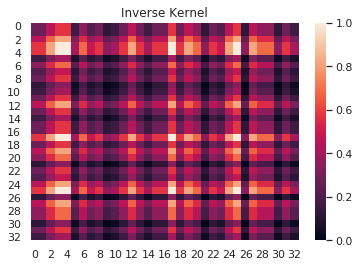
\includegraphics[width=\linewidth]{data/gram/gram.png}\par
		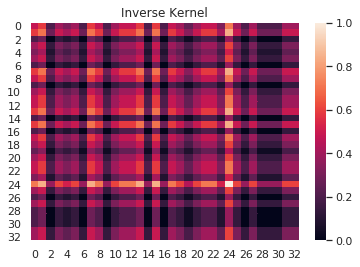
\includegraphics[width=\linewidth]{data/gram/gram2.png}\par
	\end{multicols}
	\caption{Two gram matrices computed using the Inverse Kernel on different datasets}
\end{figure}
Afterwards, in order to verify all the algorithms gave similar results, it was decided to compute the Frobenius norm of the difference of two gram matrices (divided by the size of the matrix, thus giving the mean standard deviation). The following results were obtained and were satisfying.
\begin{table}[!htb]
\begin{center}
\begin{tabular}{|p{15mm}|p{15mm}|p{15mm}|p{15mm}|p{15mm}|p{15mm}|p{15mm}|p{15mm}|}
	\hline
	& Raw\newline kernel & Inverse\newline Kernel & Sylvester\newline Equation & Conjugate\newline Gradients & Fixed\newline points & Spectral\newline Decomp. \\
	\hline
	Raw. & 0 & 1.1e-4 & 9.8e-5 & 8.9e-5 & 1.0e-4 & 1.0e-04  \\
	\hline
	Inv. & - & 0 & 2.1e-5 & 7.9e-5 & 4.0e-6 & 6.8e-6 \\
	\hline
	Syl. & - & - & 0 & 8.0e-5 & 1.7e-5 & 1.4e-5  \\
	\hline
	Con. & - & - & - & 0 & 7.9e-5 & 7.9e-5  \\
	\hline
	Fix. & - & - & - & - & 0 & 2.8e-6 \\
	\hline
	Spe. & - & - & - & - & - & 0 \\
	\hline
\end{tabular}
\end{center}
\caption {Approximate standard deviation of matrix entries (?)}
\label{tab:frobenius_norm_diff} 
\end{table}
\todo{correct nom ?}
Indeed, the 

\subsubsection{Complexity and Accuracy}

\subsubsection{title}

\subsection{Individual kernel analysis ?}
\todo{mettre ici les images variations degré d'approximation}
\subsection{Nearest Kronecker product ?}

\subsection{On molecules}

\subsection{Improvements}

\section{Conclusion and Future Work}
experiences : détailler db, tests, méthodes, les parametres, construction label, donner tableaux, resultats, teps de calculs, précision, discuter tout cela
section 4 : 1 page ou page et demi : conclusion et discussion


\appendix
\section{Appendix}
\section{Annex 1}

\section{Acknowledgements}
This work was done during the first year of my master.

\listoffigures
\listoftables
bibliographie et index

\bibliographystyle{ieeetr}
\bibliography{references}
\end{document}
